\chapter{Results}
This chapter will give results on the sensitivity of various 
input parameters of a \gls{NFC} transition scenario. 
Various types of \gls{SA} are conducted. 
The sensitivity analysis was conducted using the Dakota-\Cyclus
and Dakota-Dymond coupling. 
This chapter is broken into five main sections: 
\begin{enumerate}
    \item Sensitivity Analysis Evaluation Criteria 
    \item Transition Scenario Specification 
    \item One-at-a-time \gls{SA} results 
    \item Synergistic \gls{SA} results
    \item Global \gls{SA} results 
\end{enumerate}

\subsection{\deploy Demonstration}
\label{sec:demo}

This section will demonstrate \deploy's capability 
to effectively conduct simple transition scenario analysis
for constant, linearly increasing, and 
sinusoidal power demand simulations.
These simulations are basic transition scenarios that only include 
three types of facilities: \texttt{source}, \texttt{reactor}, and 
\texttt{sink}. 
All simulations have ten initial \texttt{reactor} facilities 
(\texttt{reactor1} to \texttt{reactor10}). 
These reactors have staggered cycle lengths and lifetimes to prevent 
simultaneous refueling and set up gradual decommissioning. 
\deploy is set up to deploy \texttt{new reactor} facilities
to meet the loss of power supply introduced from the decommissioning 
of the initial \texttt{reactor} facilities. 
The \deploy input parameters for each simulation is shown in Table 
\ref{tab:demonstrations}. 
Figure \ref{fig:powerplots} shows the user-defined power demand curves 
that \deploy needs to deploy facilities meet for each simulation.

\begin{table}[]
    \resizebox{\textwidth}{!}{%
    \begin{tabular}{|l|l|c|l|l|}
    \hline
    \multirow{2}{*}{}                         & \multicolumn{1}{c|}{\multirow{2}{*}{\textbf{Input Parameter}}} & \multicolumn{3}{c|}{\textbf{Simulation Description}}                                                                                                                                                                                                                                                       \\ \cline{3-5} 
                                              & \multicolumn{1}{c|}{}                                          & \multicolumn{1}{l|}{\textbf{Constant Power}}                                                                 & \textbf{\begin{tabular}[c]{@{}l@{}}Linearly Increasing \\ Power\end{tabular}}                  & \textbf{Sinusoidal Power}                                                                  \\ \hline
    \multirow{5}{*}{\textbf{Required Inputs}} & Demand driving commodity                                       & \multicolumn{3}{c|}{Power}                                                                                                                                                                                                                                                                                 \\ \cline{2-5} 
                                              & Demand equation                                                & \multicolumn{1}{l|}{10000 MW}                                                                                & \begin{tabular}[c]{@{}l@{}}t\textless 40: 10000 MW\\ t\textgreater{}=40: 250*t MW\end{tabular} & 1000*$\sin(\pi*t/3)$+10000                                                                 \\ \cline{2-5} 
                                              & Facilities it controls                                         & \multicolumn{3}{c|}{Source, reactor, sink}                                                                                                                                                                                                                                                                 \\ \cline{2-5} 
                                              & Prediction method                                              & \multicolumn{1}{l|}{\begin{tabular}[c]{@{}l@{}}Power: FFT\\ Fuel: MA\\ Spent fuel: MA\end{tabular}}          & \begin{tabular}[c]{@{}l@{}}Power: FFT\\ Fuel: MA\\ Spent fuel: FFT\end{tabular}                & \begin{tabular}[c]{@{}l@{}}Power: HW\\ Fuel: MA\\ Spent fuel: FFT\end{tabular}             \\ \cline{2-5} 
                                              & Deployment Driving Method                                      & \multicolumn{3}{c|}{Installed Capacity}                                                                                                                                                                                                                                                                    \\ \hline
    \multirow{2}{*}{\textbf{Optional Inputs}} & Buffer type                                                    & \multicolumn{3}{c|}{Absolute}                                                                                                                                                                                                                                                                              \\ \cline{2-5} 
                                              & Buffer size                                                    & \multicolumn{1}{l|}{\begin{tabular}[c]{@{}l@{}}Power: 3000 MW\\ Fuel: 0 kg \\ Spent fuel: 0 kg\end{tabular}} & \begin{tabular}[c]{@{}l@{}}Power: 2000 MW\\ Fuel: 1000 kg \\ Spent fuel: 0 kg\end{tabular}     & \begin{tabular}[c]{@{}l@{}}Power: 2000 MW\\ Fuel: 1000 kg \\ Spent fuel: 0 kg\end{tabular} \\ \hline
    \end{tabular}%
    }
    \caption{\deploy's input parameters for the basic transition scenarios.}
    \label{tab:demonstrations}
    \end{table}

    \begin{figure}[]
        \begin{center}
            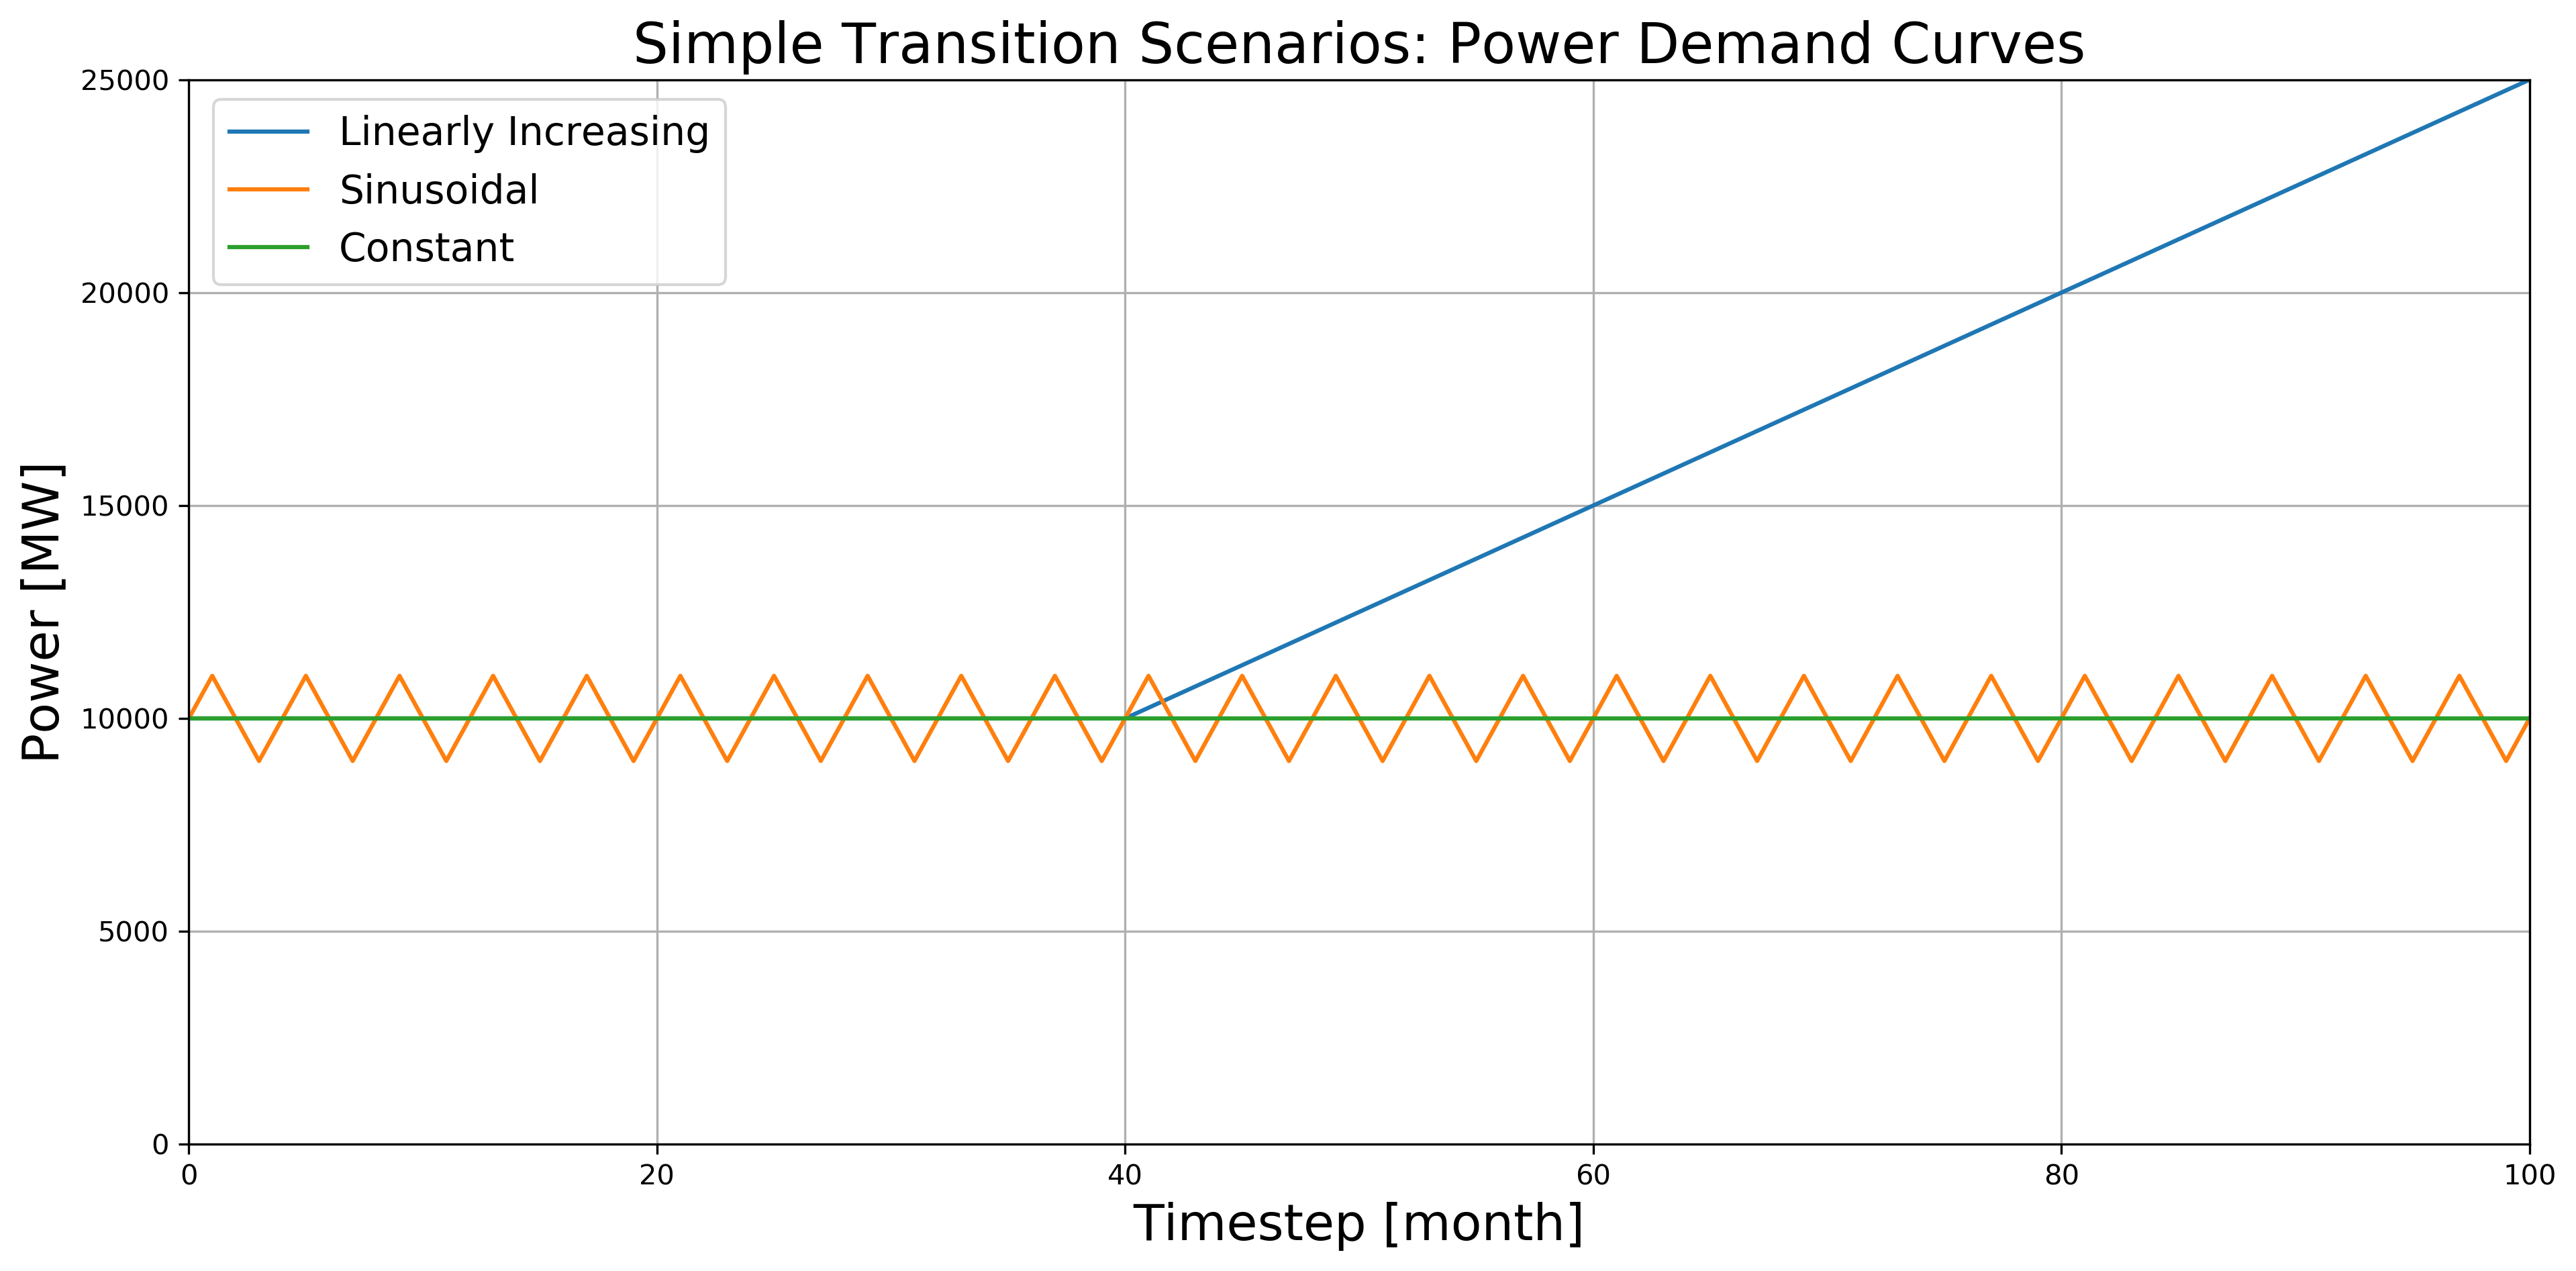
\includegraphics[scale=0.37]{./figures/powerplots.png}
        \end{center}
            \caption{Power demand curves for basic transition scenarios.}
        \label{fig:powerplots}
    \end{figure}

\subsubsection{\textbf{Basic Transition Scenario Simulation: Constant Demand}}
Figures \ref{fig:constanttransition-power}, \ref{fig:constanttransition-fuel}
and \ref{fig:constanttransition-spentfuel} demonstrate \deploy's capability 
to deploy reactor and supporting facilities to meet the user 
determined constant power demand and subsequently demanded 
secondary commodities with minimal undersupply. 
Table \ref{tab:transition-scenario-results} shows the number of 
undersupplied timesteps. 
Figure \ref{fig:constanttransition-power} demonstrates that
the main objective of \deploy (section \ref{sec:d3ploy}) 
was met since there are no timesteps
in which the supply of power falls under demand.
By using a combination of the fast fourier transform method for 
predicting demand and setting the supply buffer to 3000MW 
(the capacity of 3 reactors), the user minimizes the number of 
undersupplied timesteps for every commodity.

In figure \ref{fig:constanttransition-fuel},
a facility with a large fuel throughput is initially
deployed to meet the large initial fuel demand for the starting
up of ten reactors. 
\deploy is prevented from deploying many supporting
facilities that end up being redundant at the later parts of 
the simulation, by having an initial facility with a large throughput
exist for the first few timesteps in the simulation.
This is a reflection of reality in which reactor manufacturers will 
accumulate an appropriate amount of fuel inventory before starting 
up reactors. 
There is one timestep where there is an undersupply after the 
decommissioning of the large initial facility.  
This is unavoidable since the prediction methods in \deploy are 
unable to predict this sudden drop in demand. 

    \begin{figure}[]
        \centering
        \begin{subfigure}[t]{\textwidth}
        \centering
            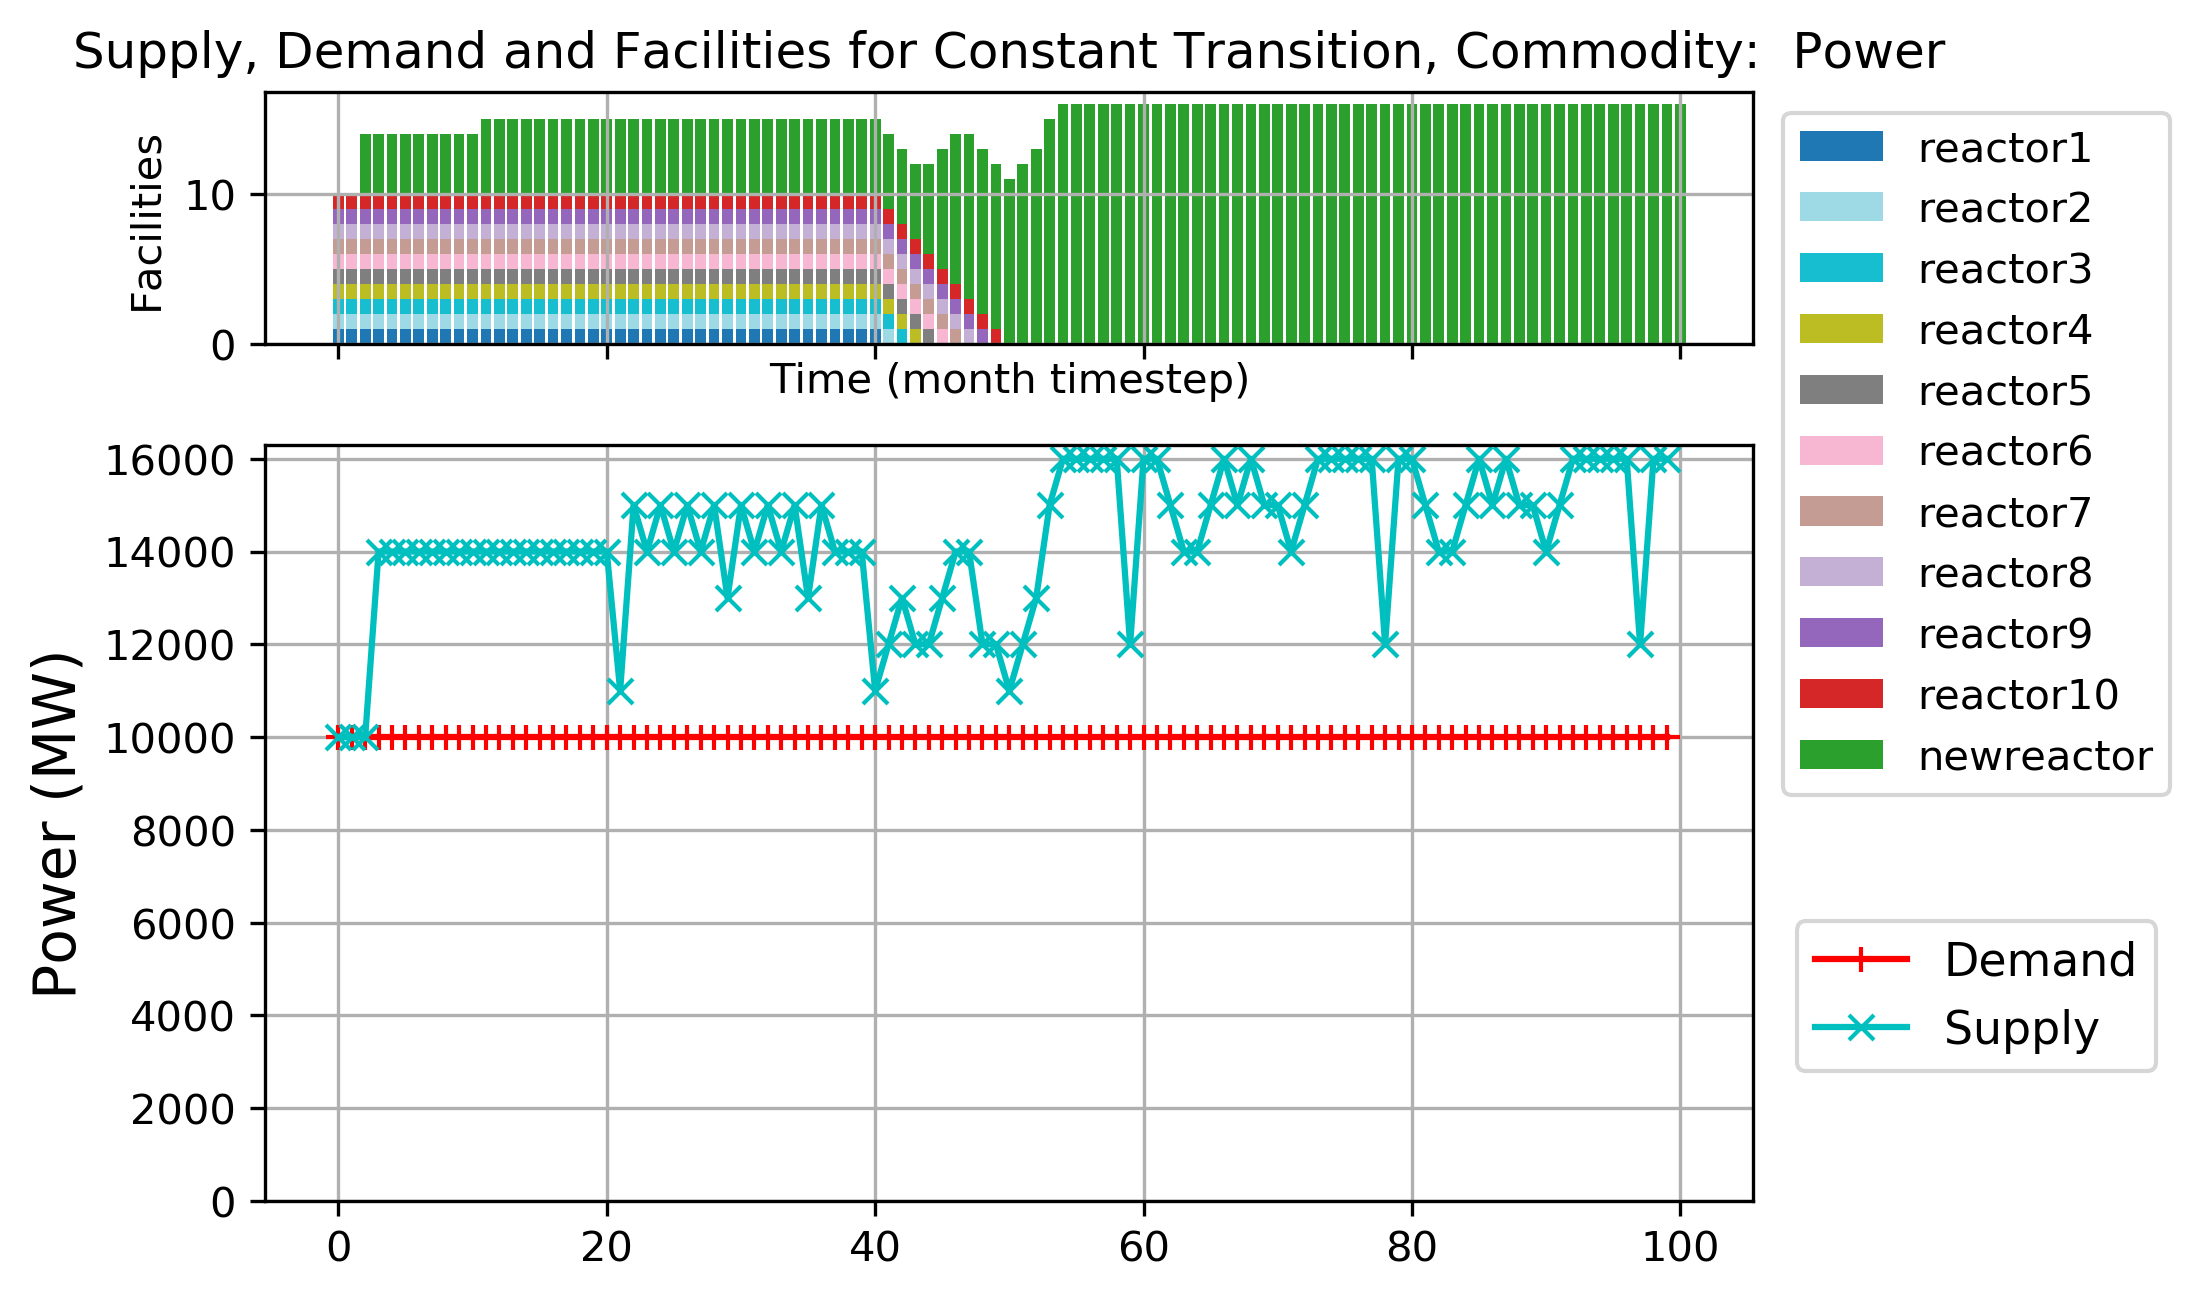
\includegraphics[width=0.7\linewidth]{figures/constanttransition-power.png} 
            \caption{The power demand is a user-defined equation and power is supplied by the reactors.}
            \label{fig:constanttransition-power}
        \end{subfigure}
        \begin{subfigure}[t]{0.6\textwidth}
            \centering
            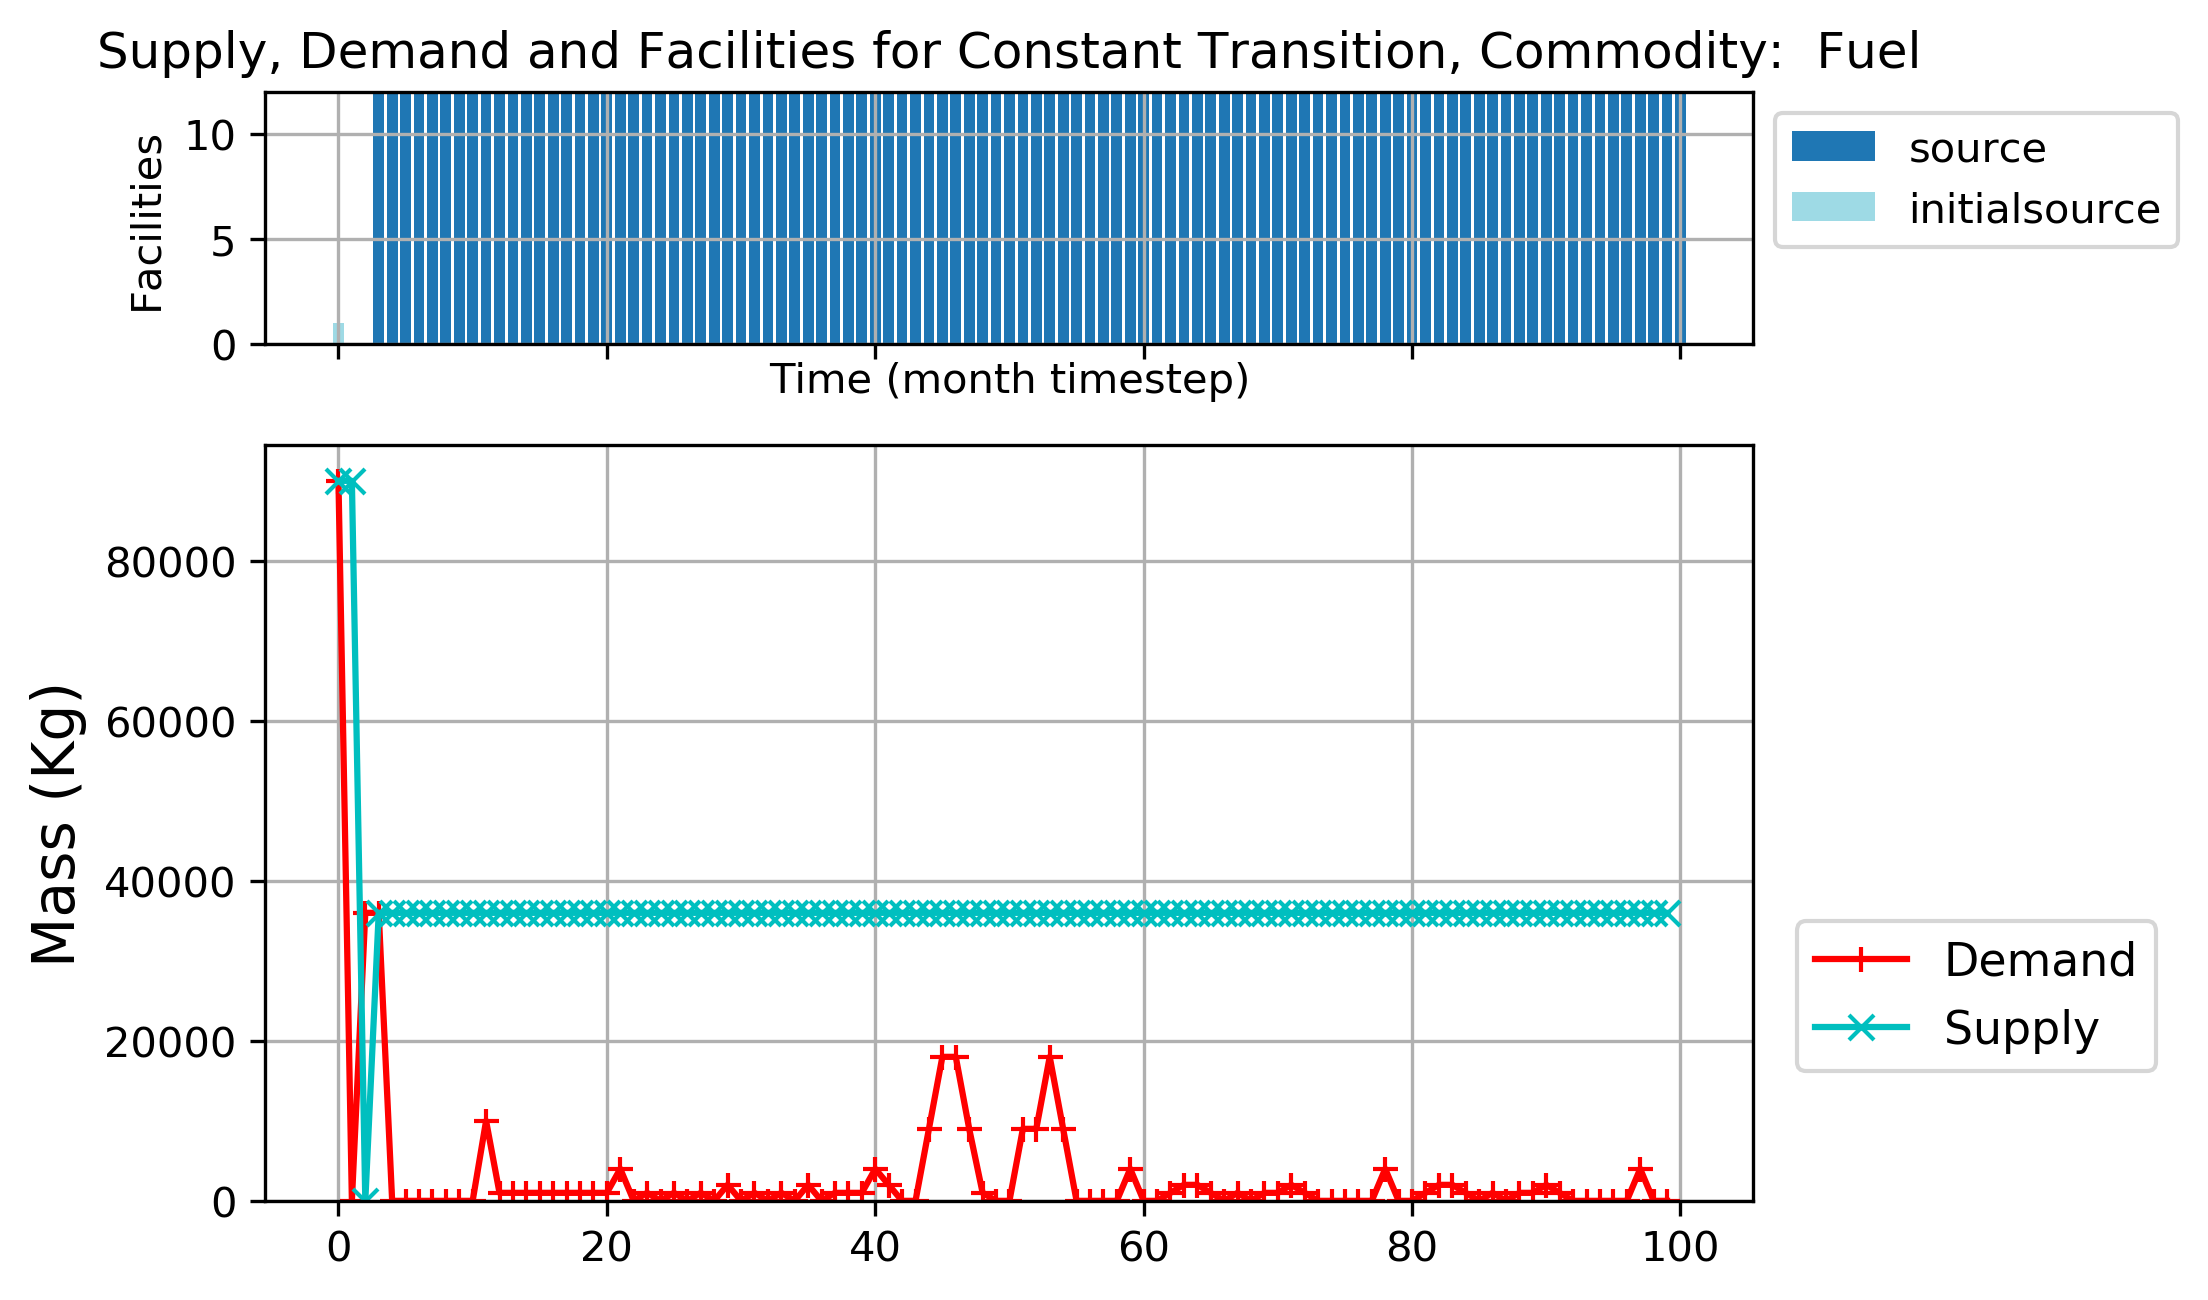
\includegraphics[width=\linewidth]{figures/constanttransition-fuel.png} 
            \caption{Fuel is demanded by reactors and supplied by source facilities.}
            \label{fig:constanttransition-fuel}
        \end{subfigure}
        \begin{subfigure}[t]{0.6\textwidth}
            \centering
            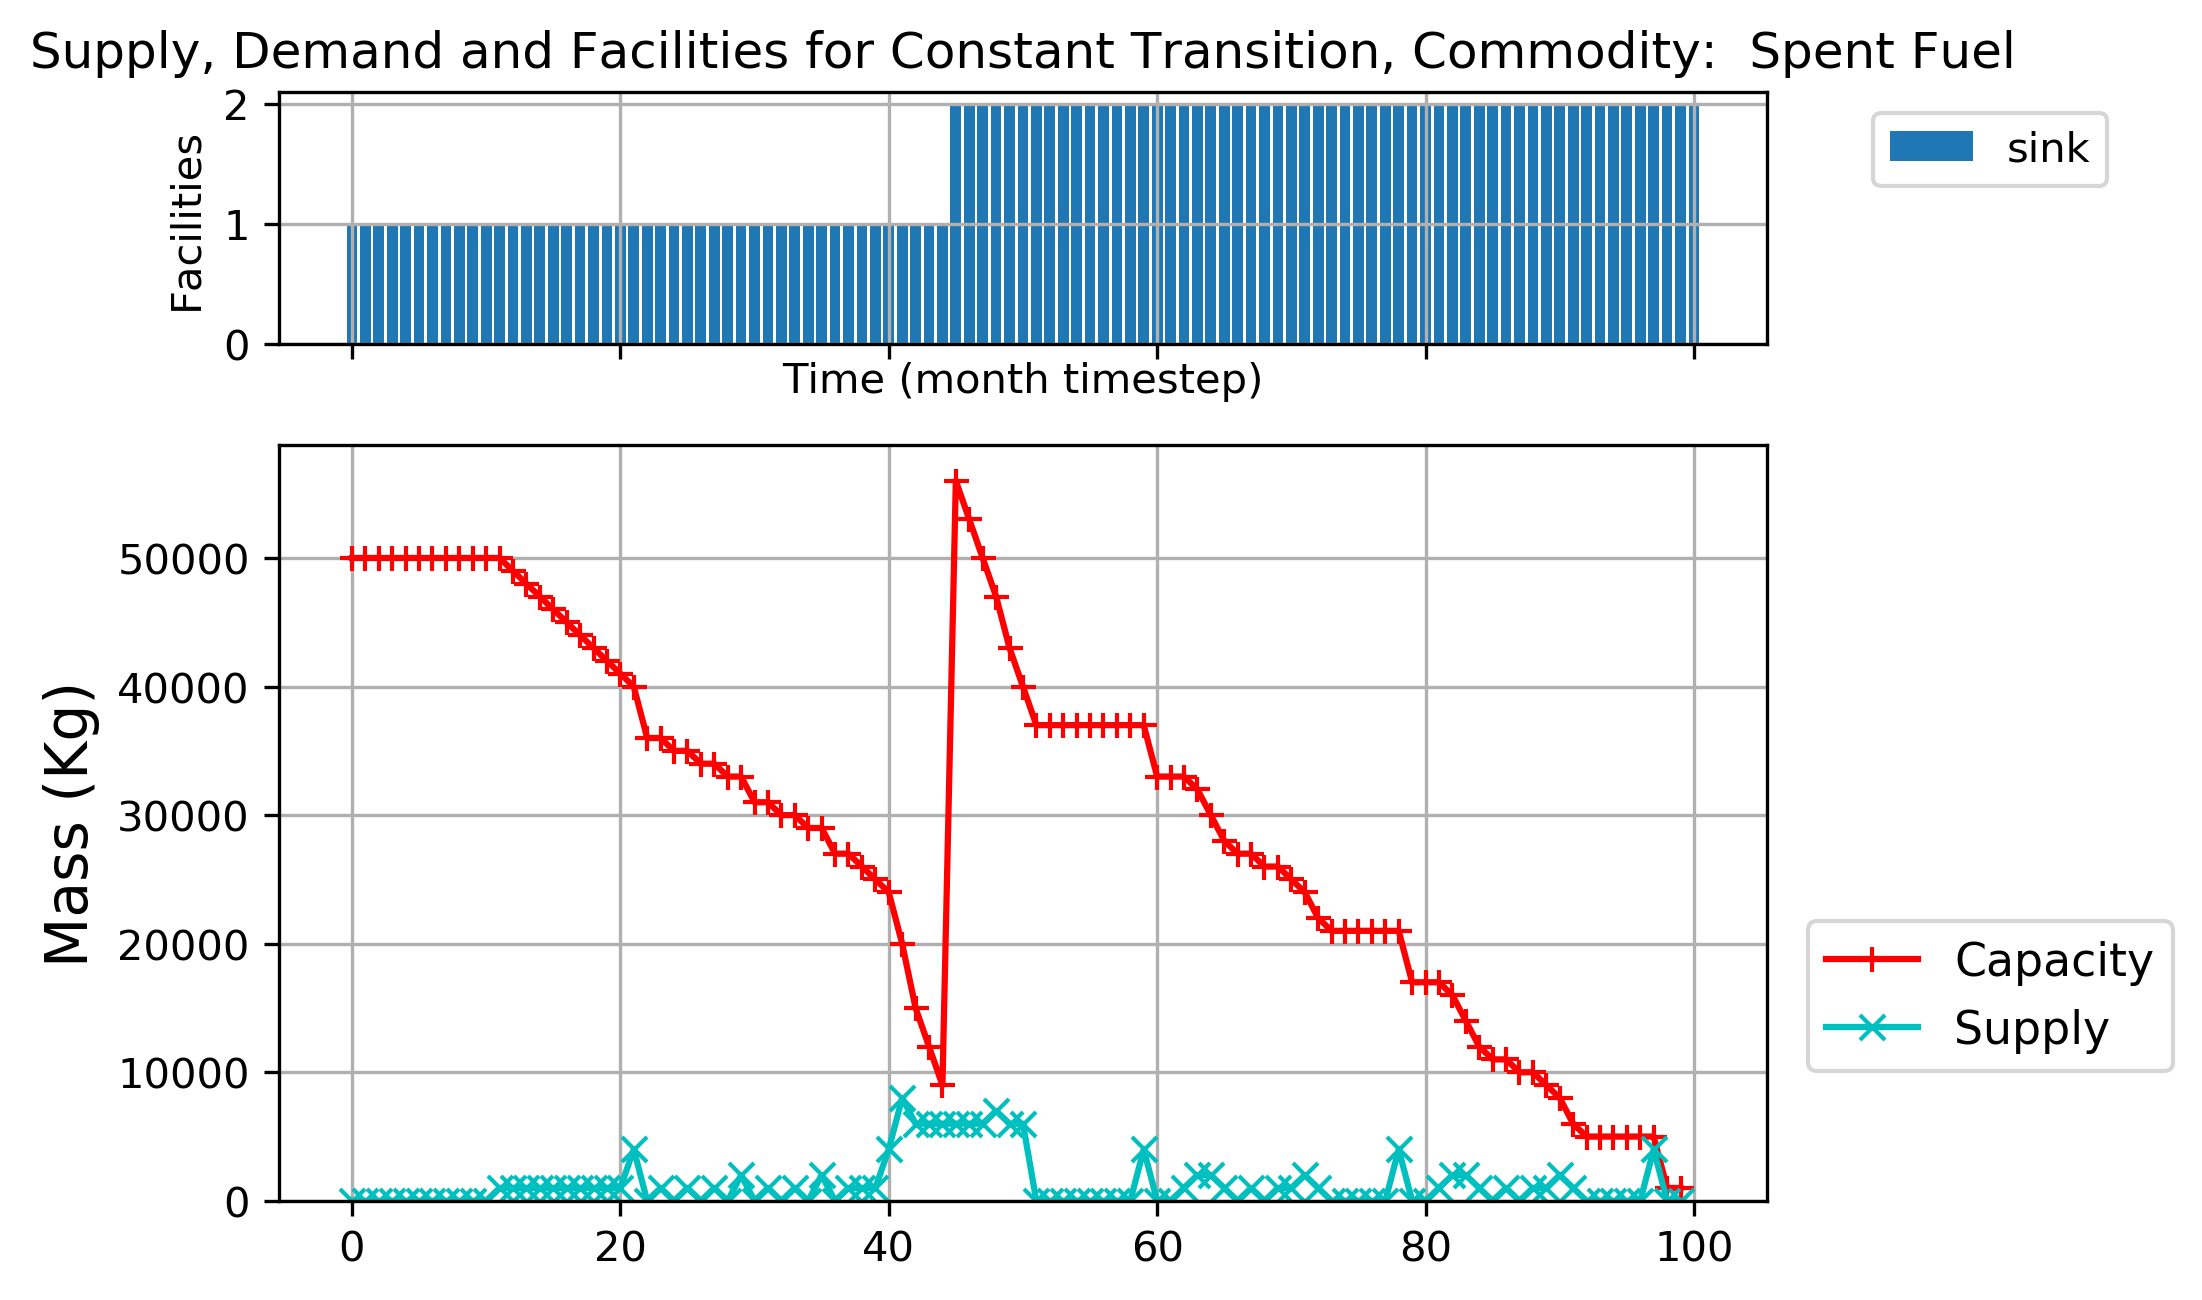
\includegraphics[width=\linewidth]{figures/constanttransition-spentfuel.png} 
            \caption{Spent Fuel is supplied by reactors and the capacity is provided by sink facilities.}
            \label{fig:constanttransition-spentfuel}
        \end{subfigure}
        \caption{Transition Scenario: Constant Power Demand of 10000MW}
    \end{figure}

    \subsubsection{\textbf{Basic Transition Scenario Simulation: Linearly Increasing Demand}}

    Figures \ref{fig:growingtransition-power}, \ref{fig:growingtransition-fuel}
    and \ref{fig:growingtransition-spentfuel} demonstrate the capability 
    of \deploy to deploy reactor and supporting facilities to meet the
    power demand and subsequently demanded secondary commodities 
    for a linearly increasing power demand. 
    A smaller supply buffer could be used while still minimizing under supply.
    Table \ref{tab:transition-scenario-results} shows the number of 
    undersupplied timesteps. 
    Figure \ref{fig:growingtransition-power} demonstrates that
    the main objective of \deploy (section \ref{sec:d3ploy}) 
    was met since there are no timesteps
    in which the supply of power falls under demand.
    
    \begin{figure}[]
        \centering
        \begin{subfigure}[t]{\textwidth}
        \centering
            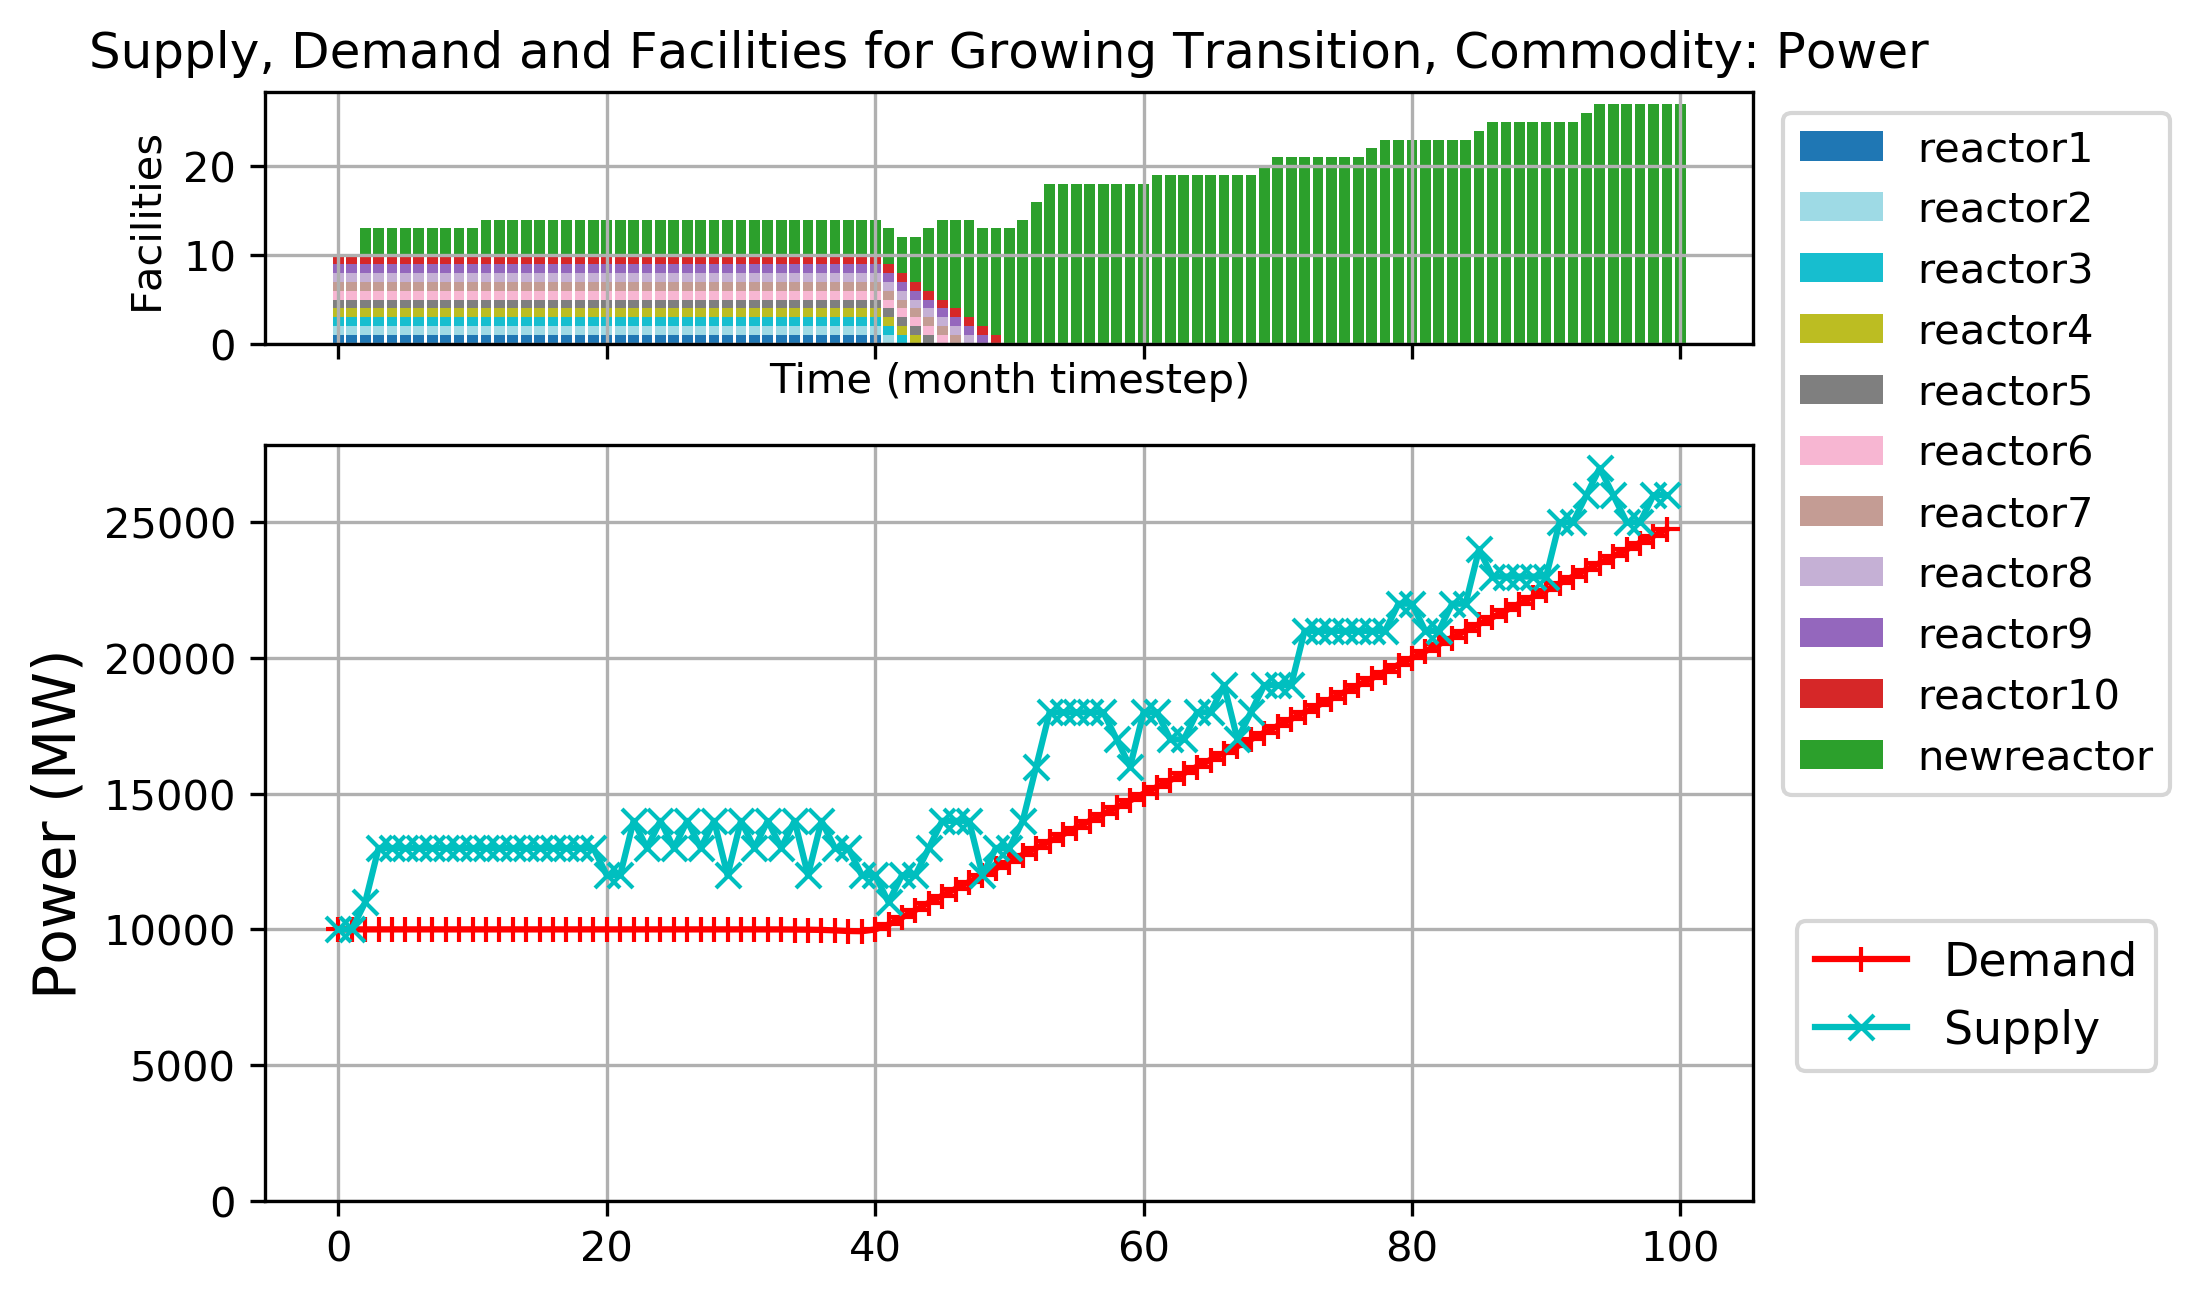
\includegraphics[width=0.7\linewidth]{figures/growingtransition-power.png} 
            \caption{The power demand is a user-defined equation and power is supplied by the reactors.}
            \label{fig:growingtransition-power}
        \end{subfigure}
        \begin{subfigure}[t]{0.6\textwidth}
            \centering
            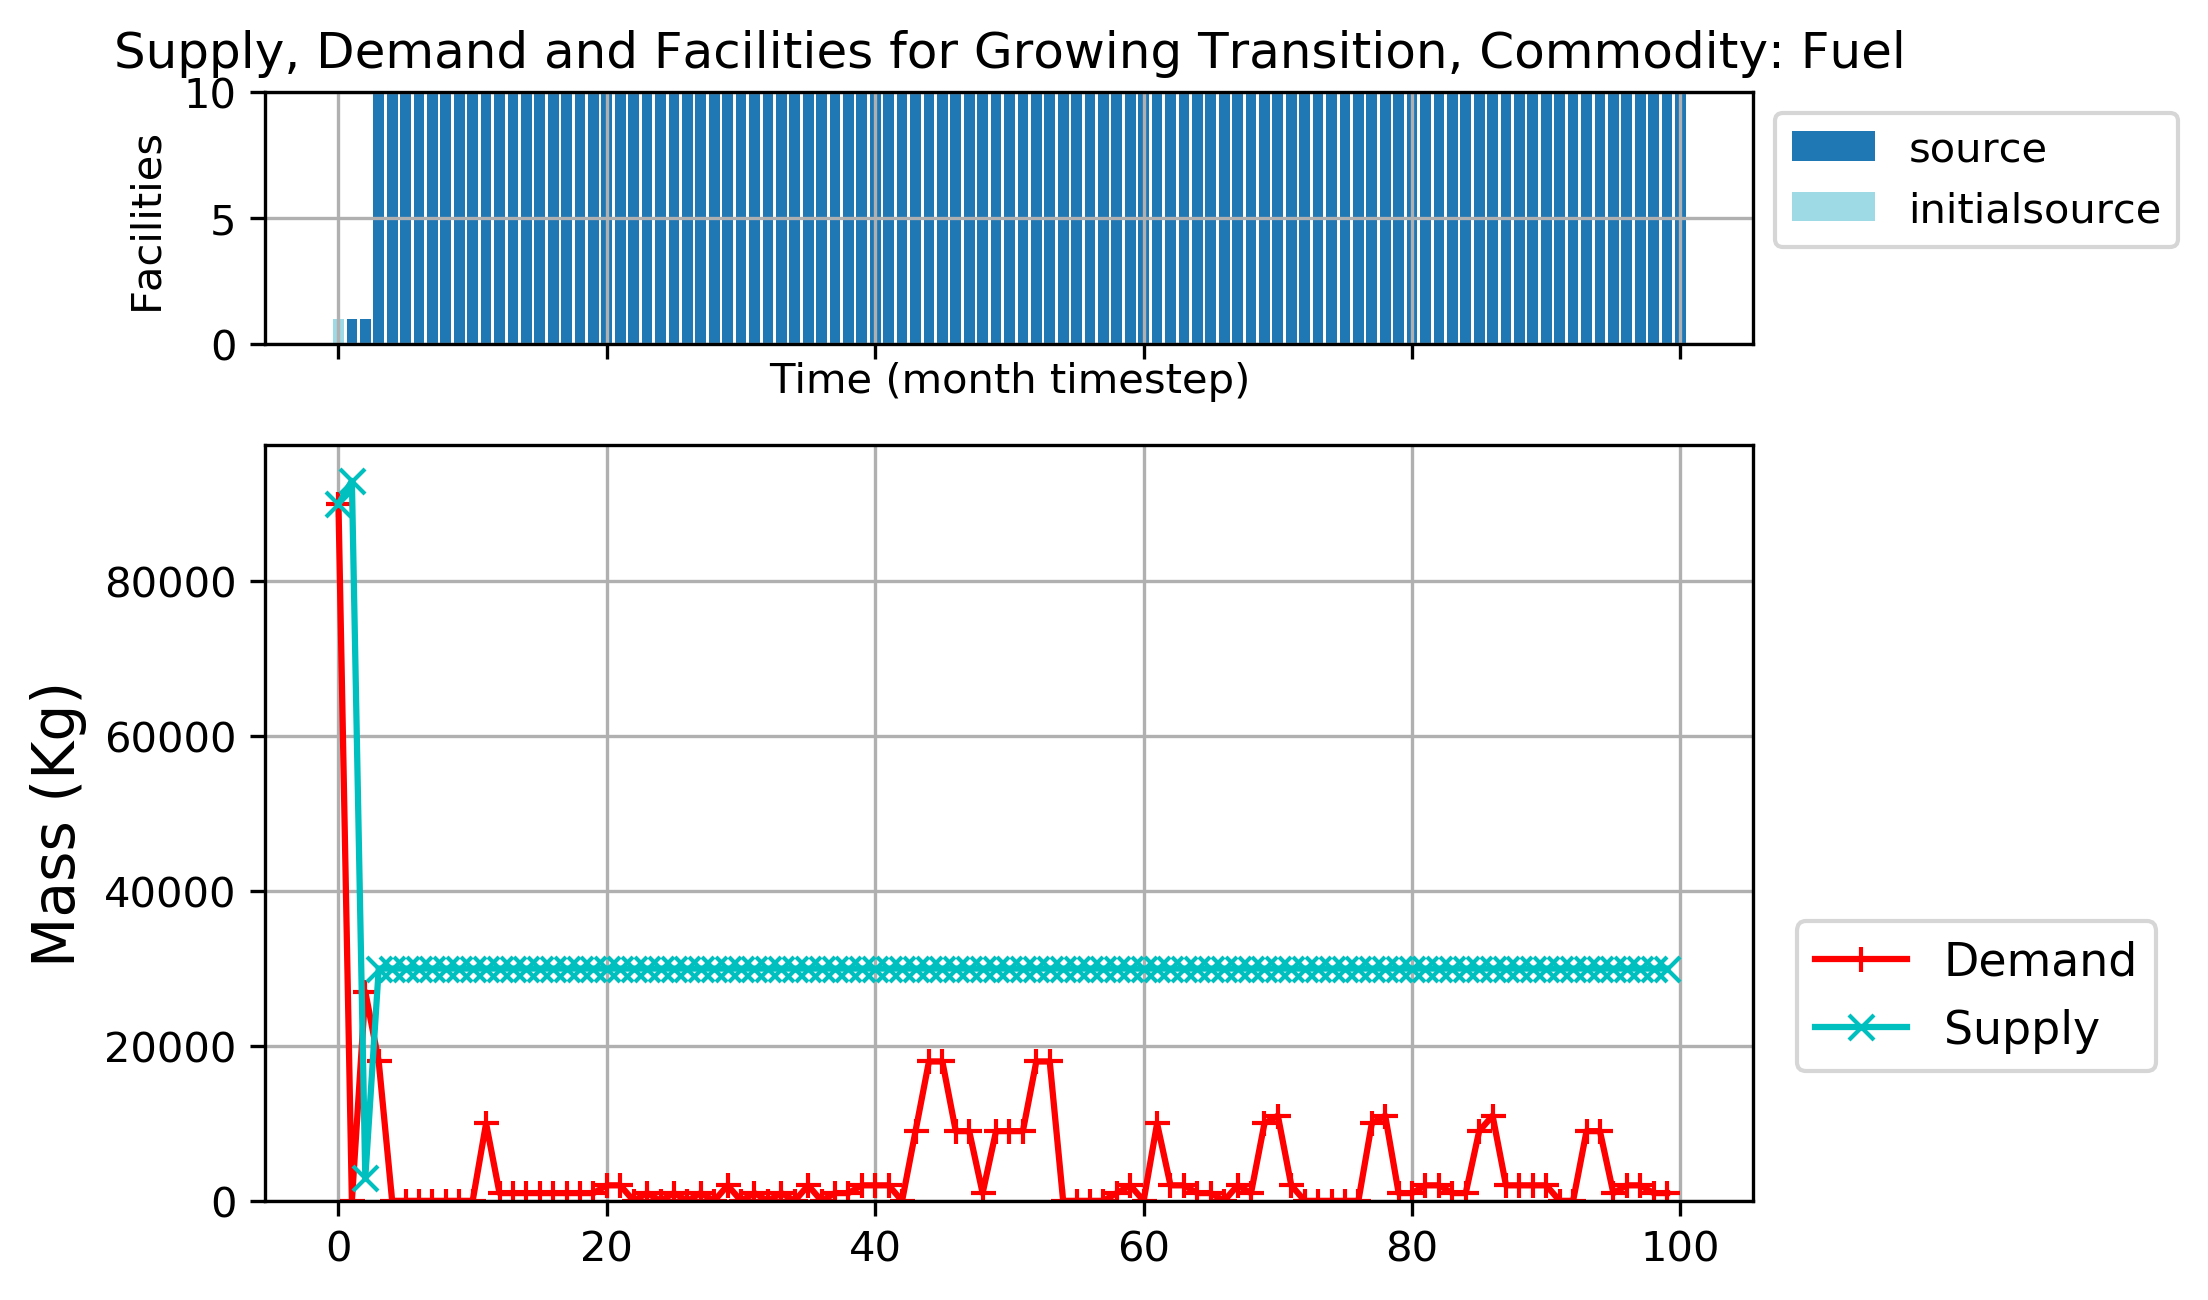
\includegraphics[width=\linewidth]{figures/growingtransition-fuel.png} 
            \caption{Fuel is demanded by reactors and supplied by source facilities.}
            \label{fig:growingtransition-fuel}
        \end{subfigure}
        \begin{subfigure}[t]{0.6\textwidth}
            \centering
            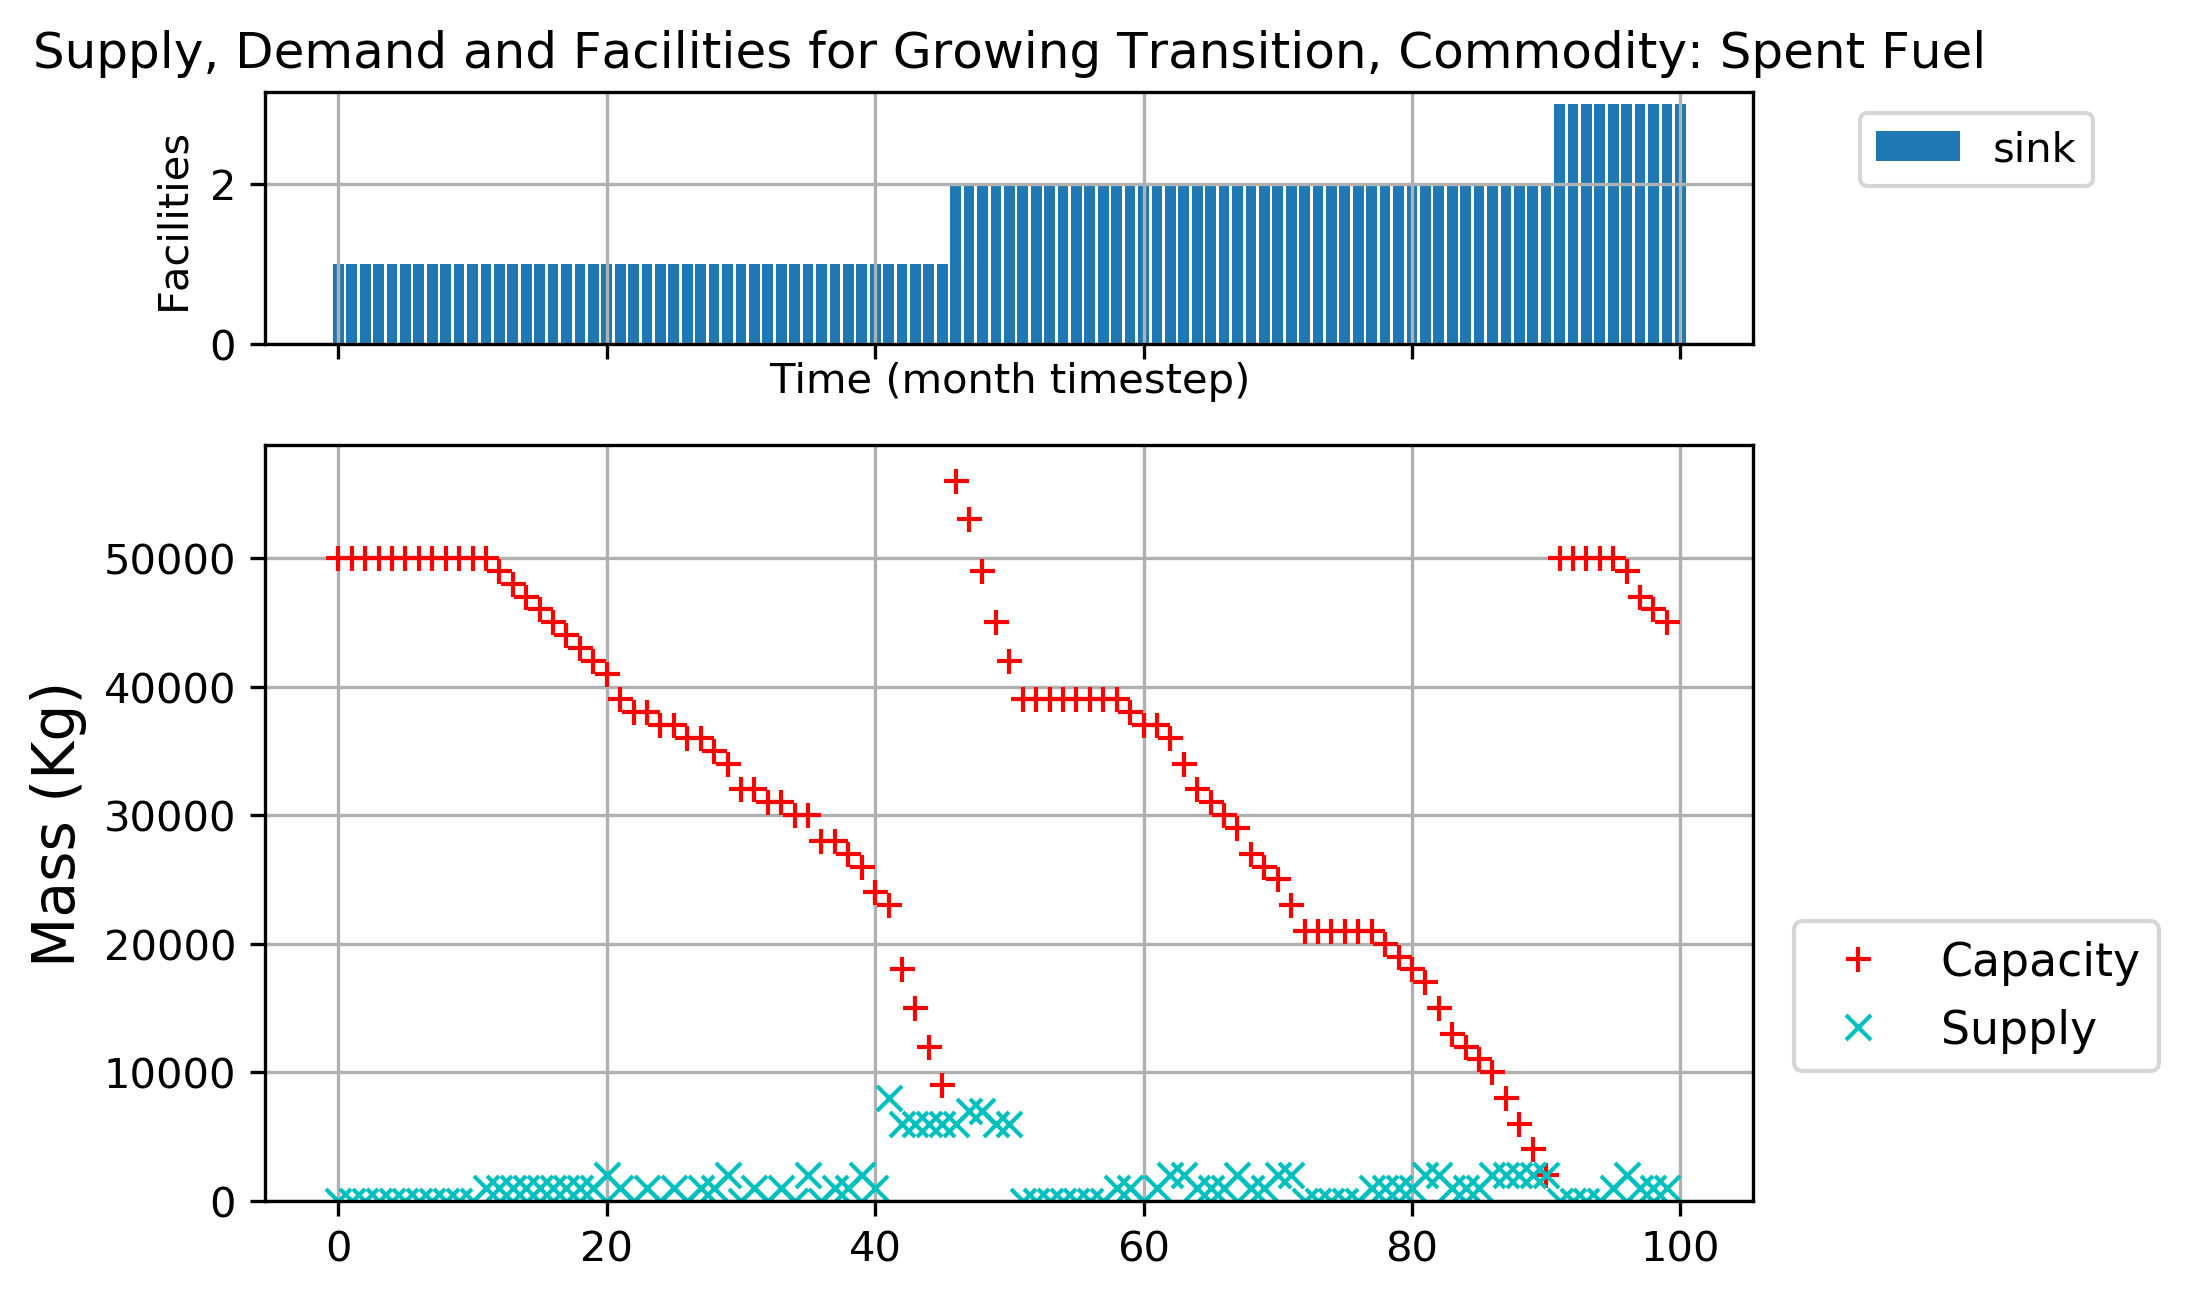
\includegraphics[width=\linewidth]{figures/growingtransition-spentfuel.png} 
            \caption{Spent Fuel is supplied by reactors and the capacity is provided by sink facilities.}
            \label{fig:growingtransition-spentfuel}
        \end{subfigure}
        \caption{Transition Scenario: Linearly Increasing Power Demand.}
    \end{figure}
    
    \subsubsection{\textbf{Basic Transition Scenario Simulation: Sinusoidal Demand}}
    A sinusoidal power demand is the reflection of power demand in 
    the real world where power usage is higher in the winter and summer
    and lower in the spring and fall. 
    Figures \ref{fig:sinetransition-power}, \ref{fig:sinetransition-fuel}
    and \ref{fig:sinetransition-spentfuel} demonstrate the capability 
    of \deploy to deploy reactor and supporting facilities to meet the
    power demand and subsequently demanded secondary commodities 
    for a sinusoidal power demand. 
    Table \ref{tab:transition-scenario-results} shows the number of 
    undersupplied timesteps.
    
    For a sinusoidal power demand, the use of the triple exponential method
    for predicting demand is more effective than the 
    fast fourier transform method which was used for the constant 
    and linearly increasing power demand transition scenarios. 
    This is because the triple exponential smoothing method excels in
    forecasting data points for repetitive seasonal series of data. 
    
    \begin{figure}[]
        \centering
        \begin{subfigure}[t]{\textwidth}
        \centering
            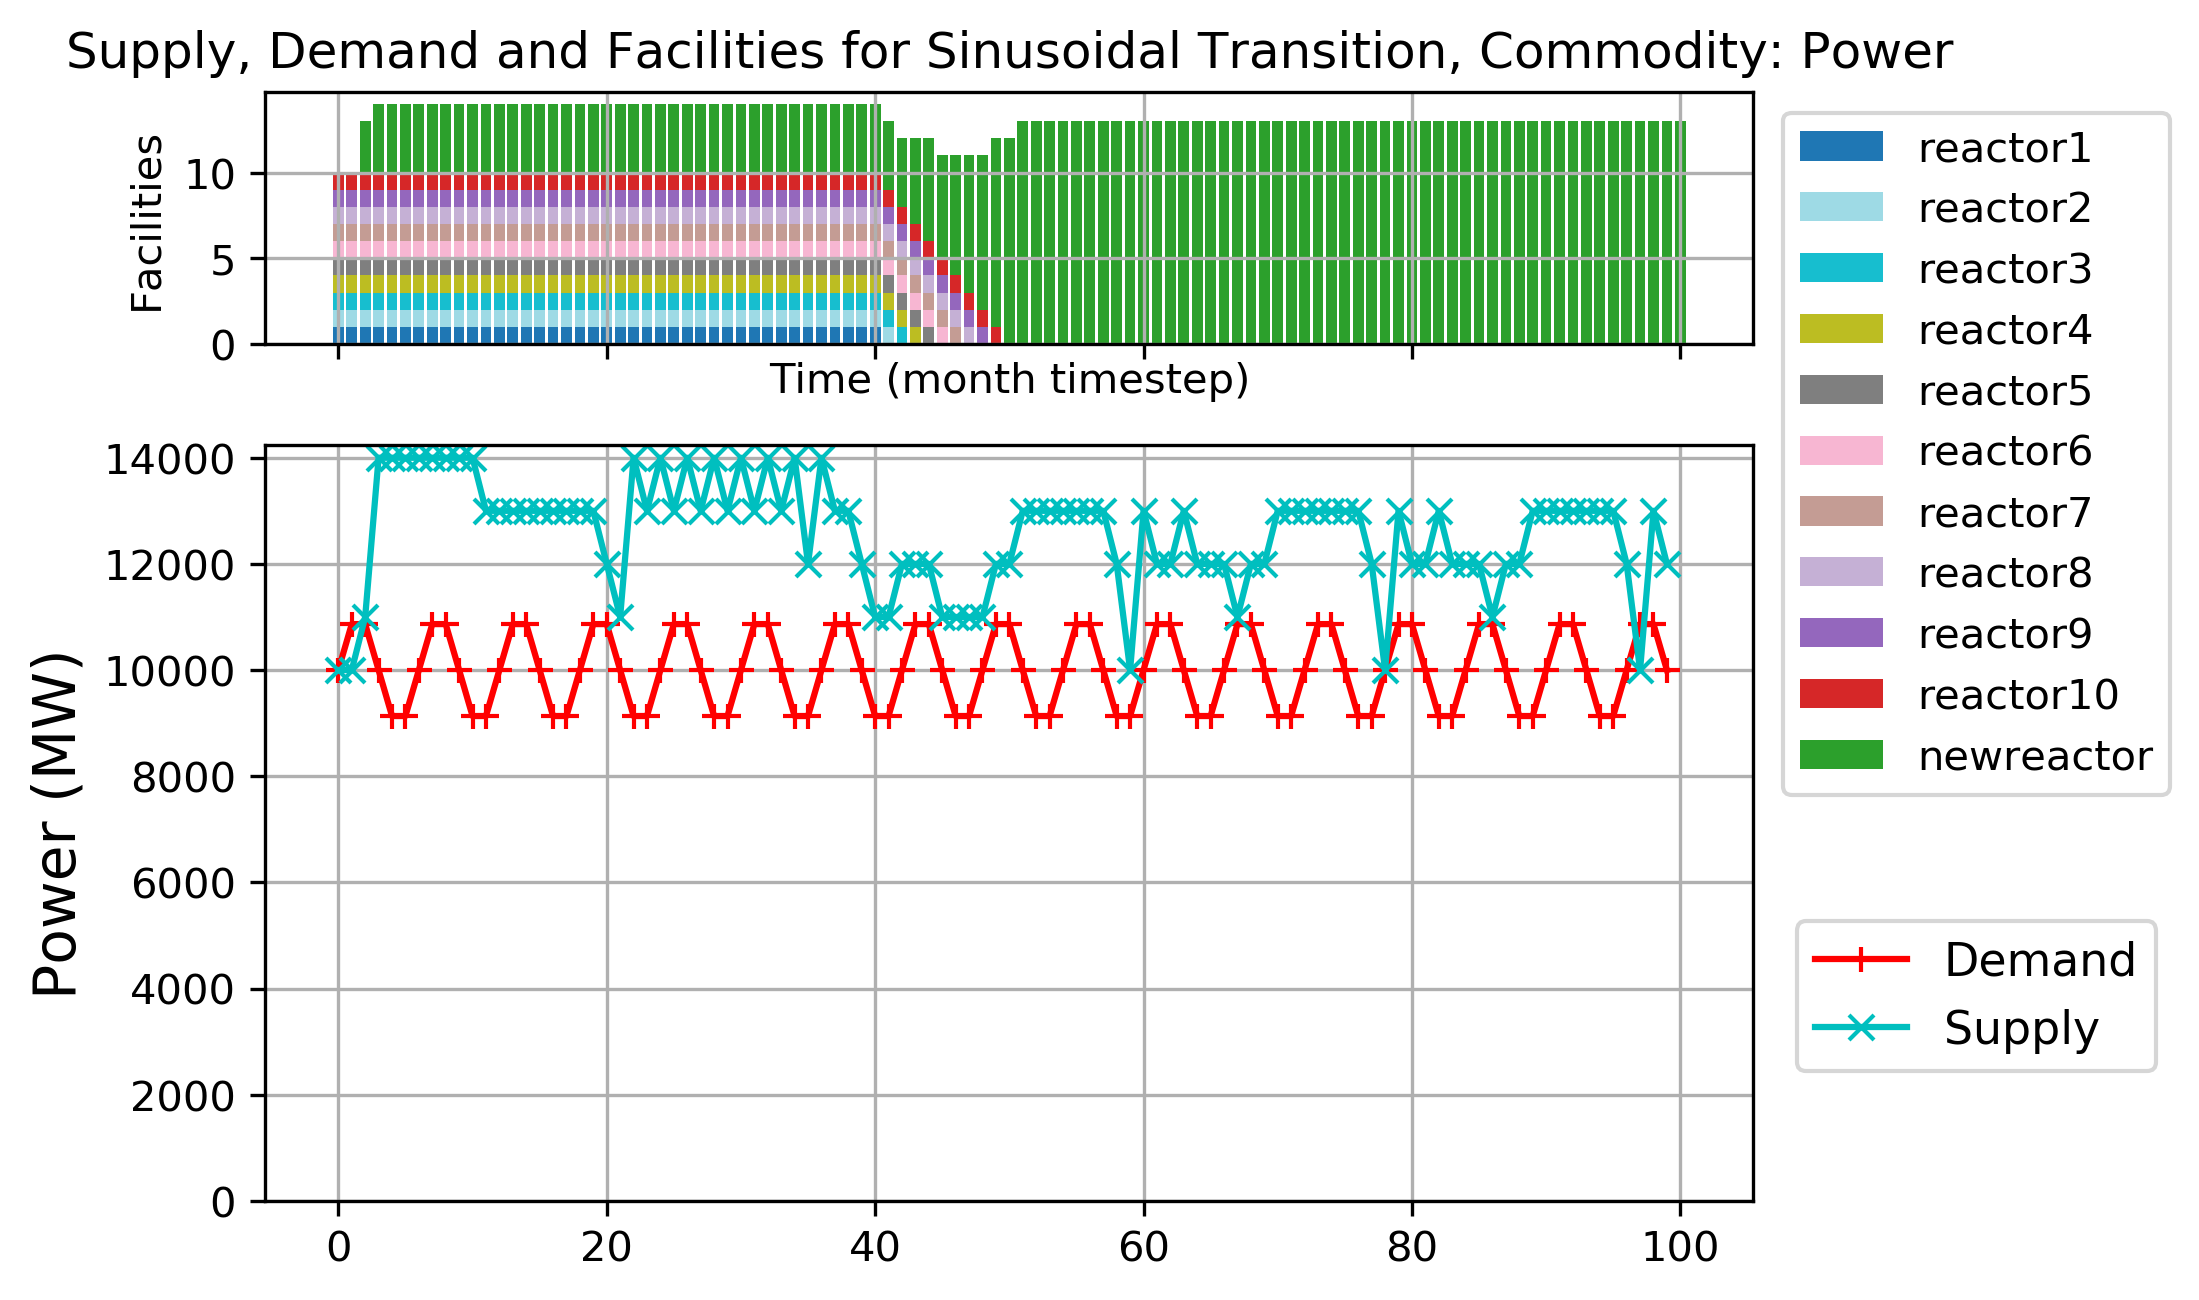
\includegraphics[width=0.7\linewidth]{figures/sinetransition-power.png} 
            \caption{The power demand is a user-defined equation and power is supplied by the reactors.}
            \label{fig:sinetransition-power}
        \end{subfigure}
        \begin{subfigure}[t]{0.6\textwidth}
            \centering
            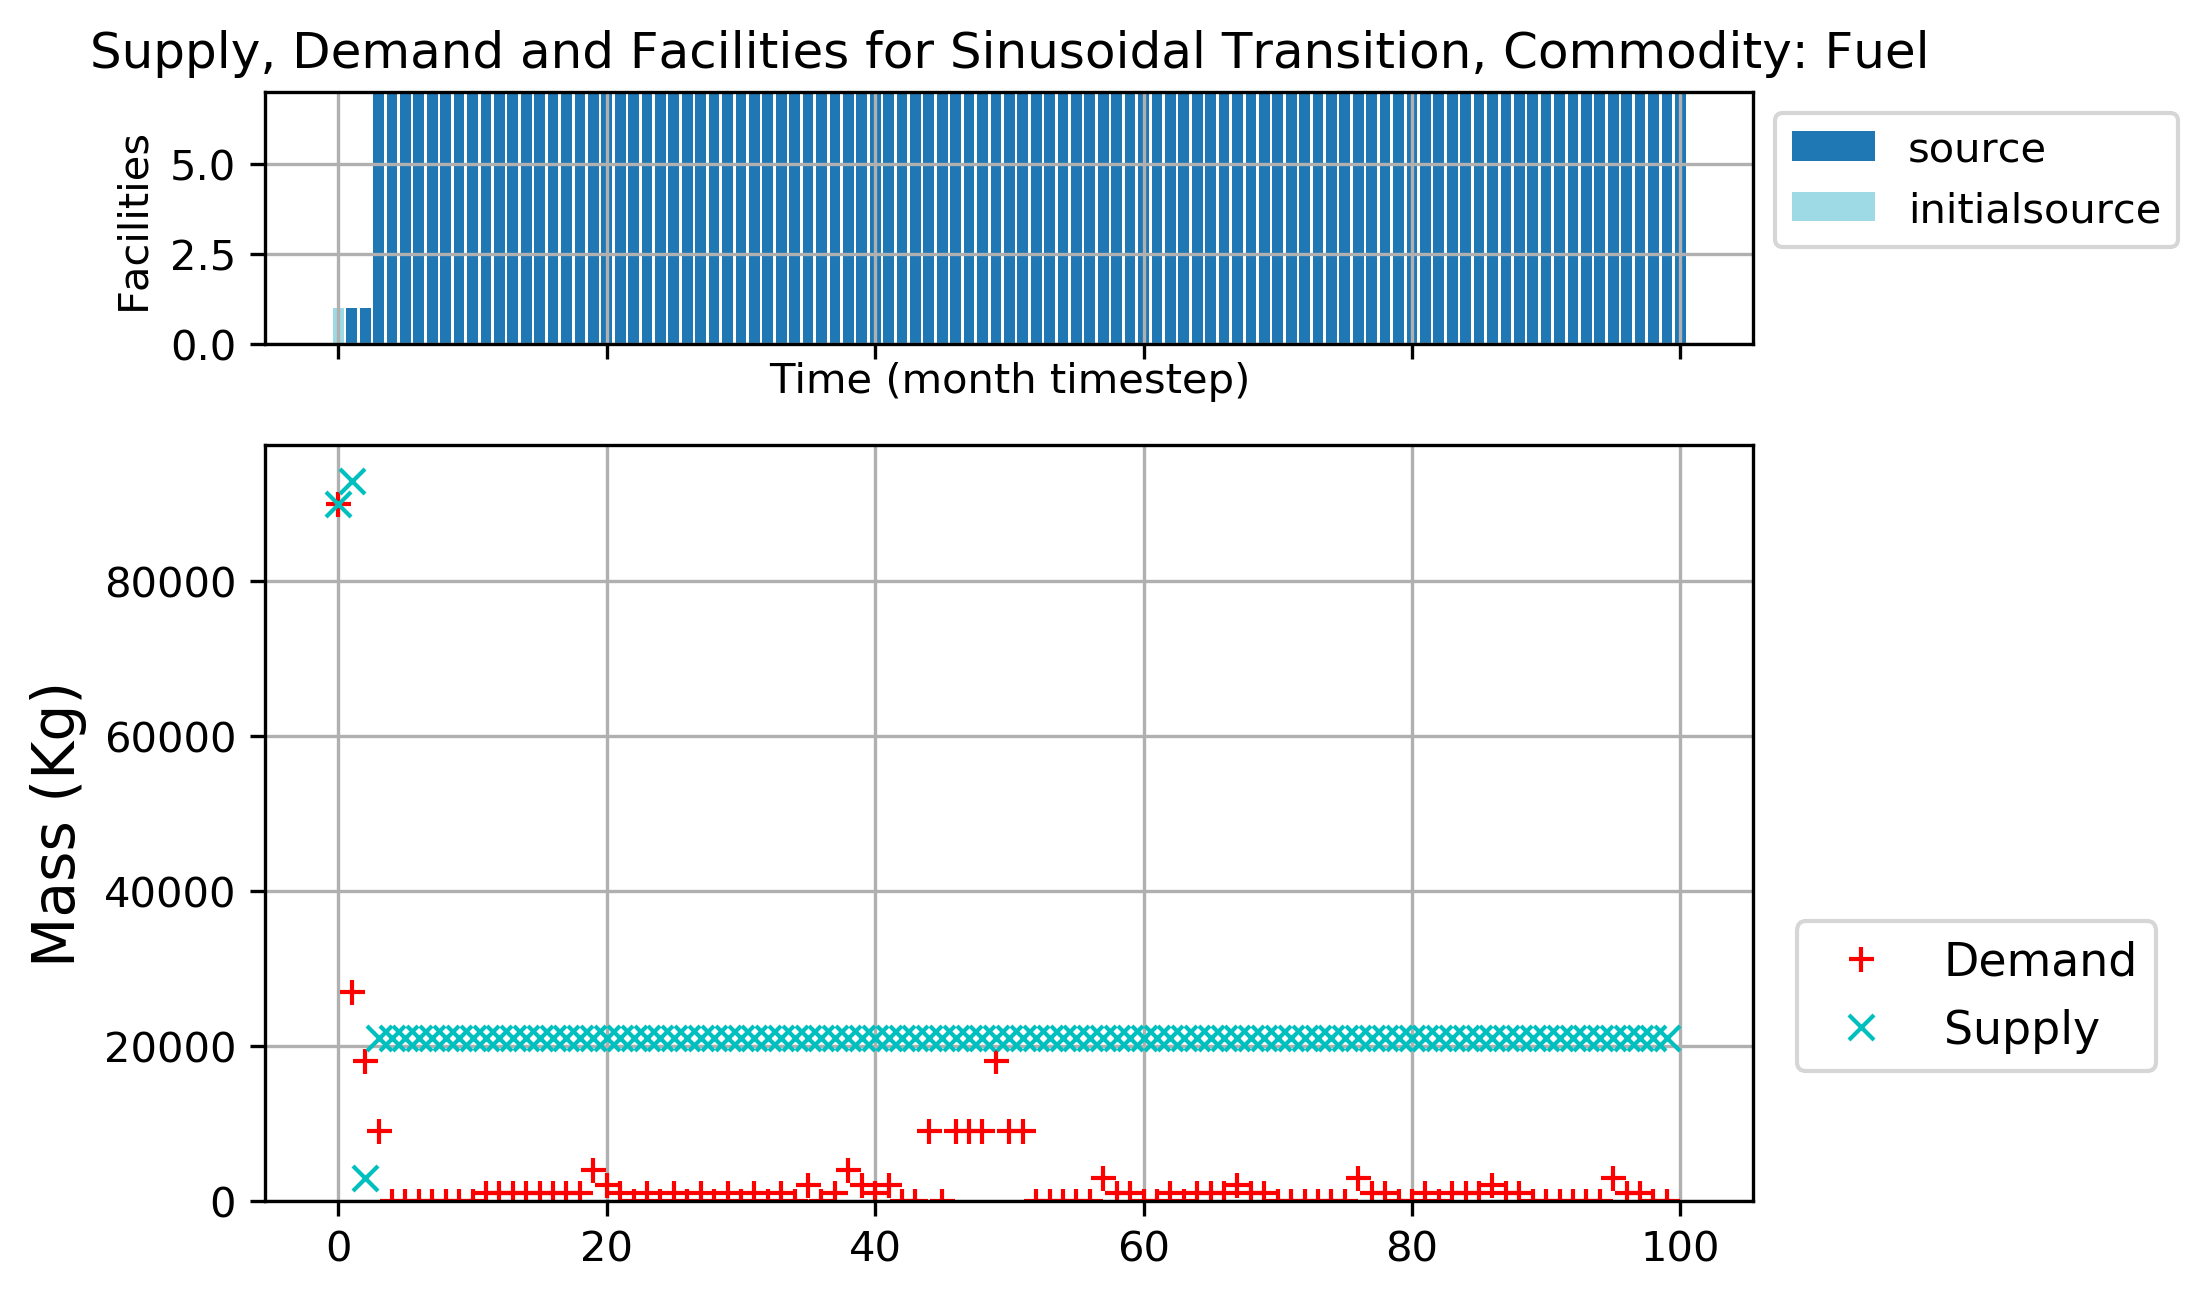
\includegraphics[width=\linewidth]{figures/sinetransition-fuel.png} 
            \caption{Fuel is demanded by reactors and supplied by source facilities.}
            \label{fig:sinetransition-fuel}
        \end{subfigure}
        \begin{subfigure}[t]{0.6\textwidth}
            \centering
            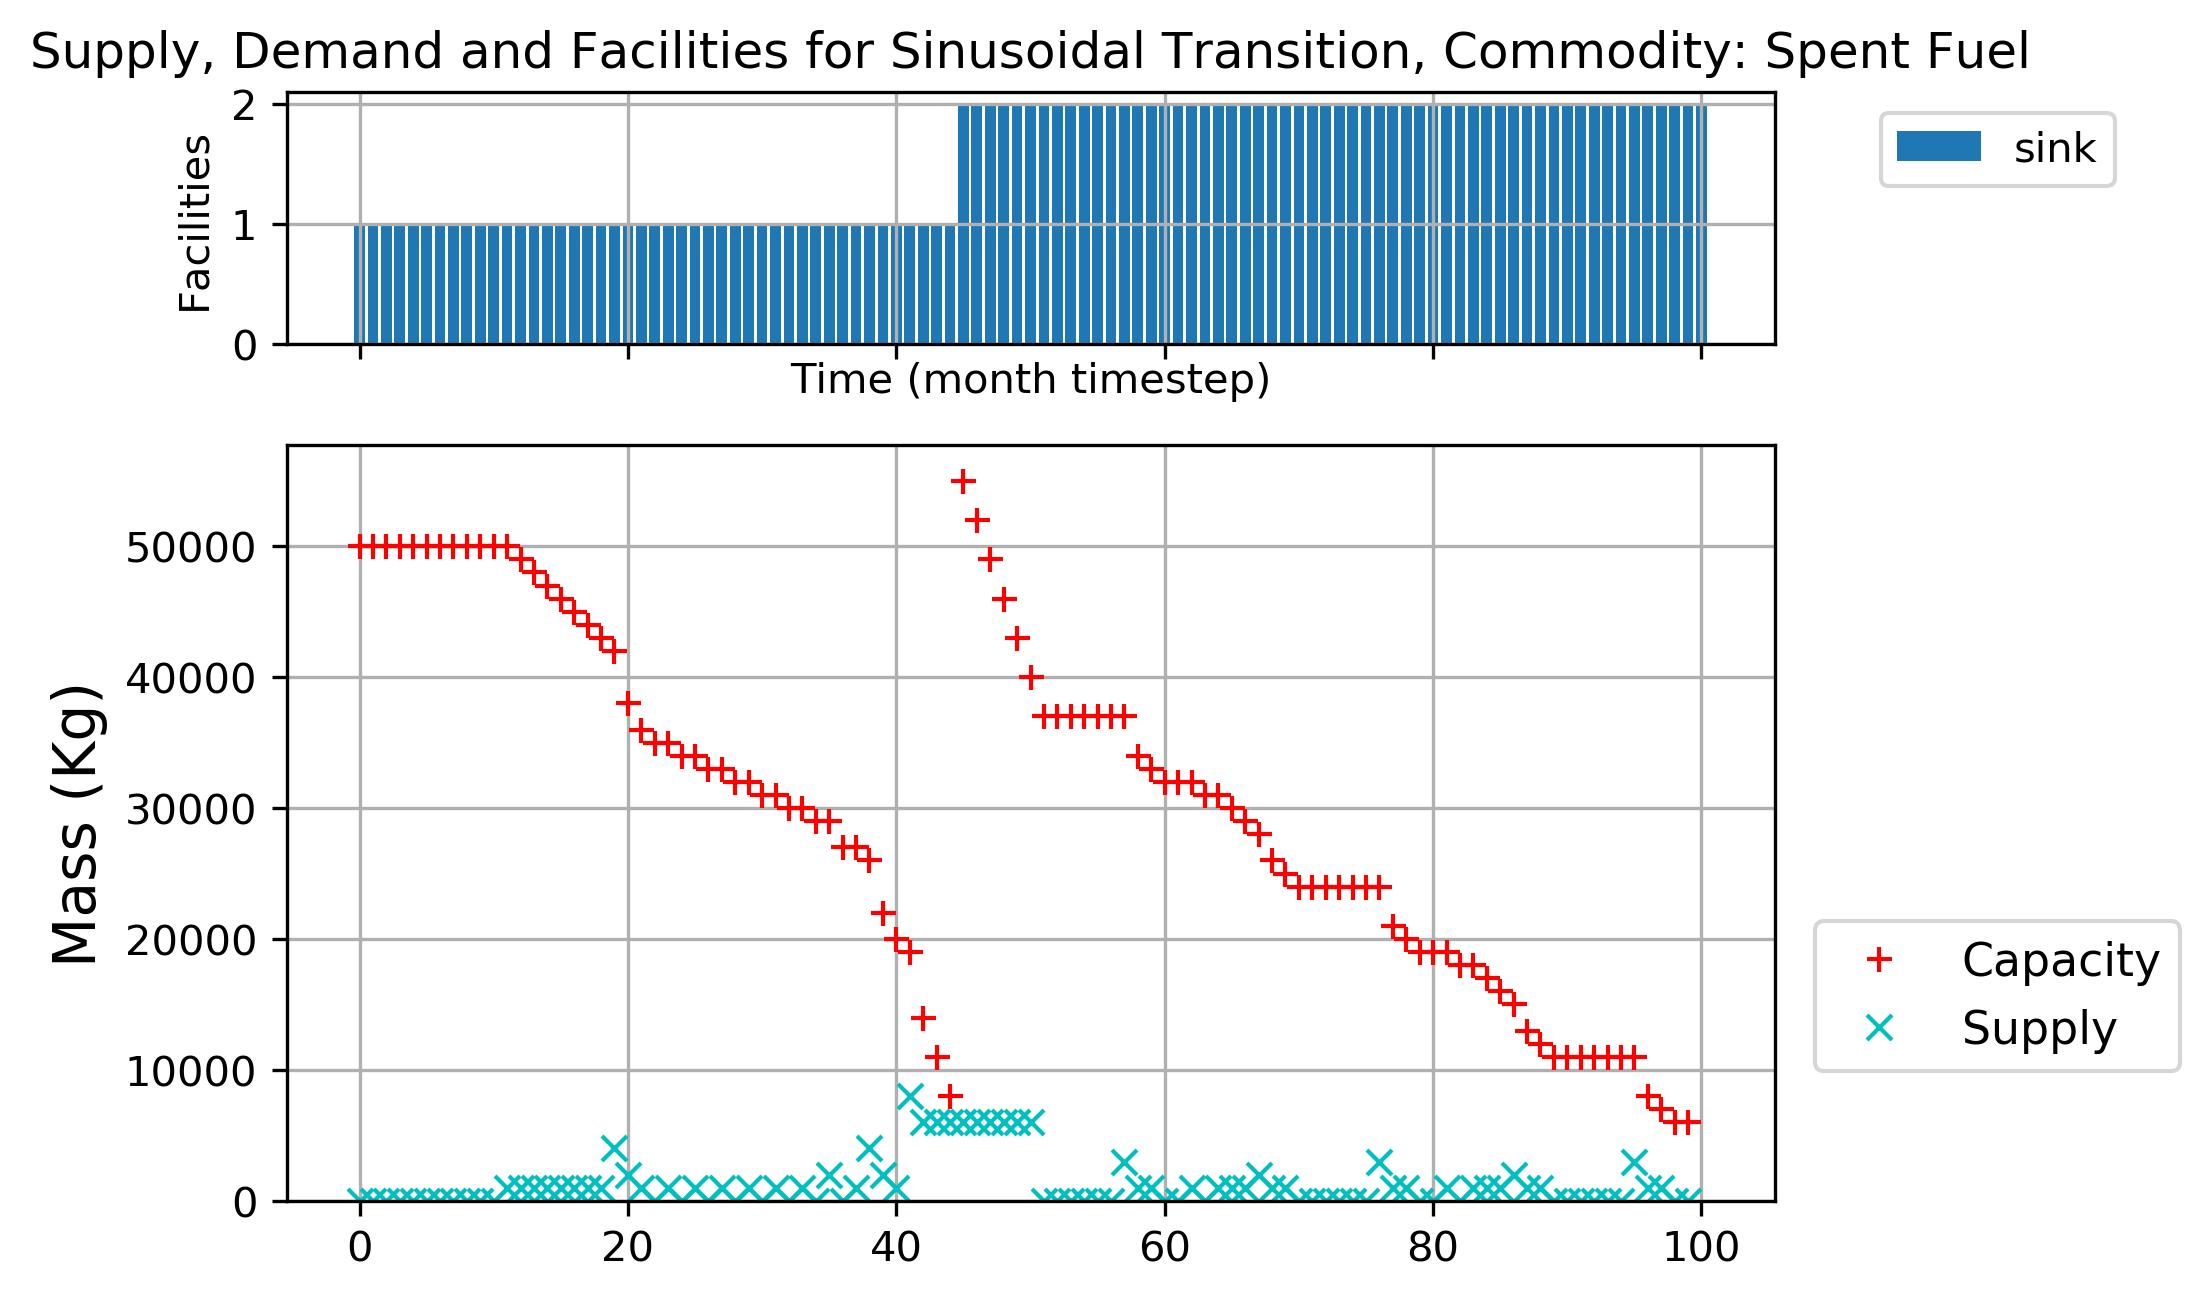
\includegraphics[width=\linewidth]{figures/sinetransition-spentfuel.png} 
            \caption{Spent Fuel is supplied by reactors and the capacity is provided by sink facilities.}
            \label{fig:sinetransition-spentfuel}
        \end{subfigure}
        \caption{Transition Scenario: Sinusoidal Power Demand}
    \end{figure}

    \begin{table}[]
        \centering
        \caption {Undersupply results for each commodity in each scenario}
        \label{tab:transition-scenario-results}
            \footnotesize
            \begin{tabularx}{\textwidth}{l|LL}	
                \hline
                \textbf{Basic Transition Scenario}    & \textbf{Commodity}    & \textbf{No. of timesteps with undersupply} \\ \hline
                \multirow{2}{*}{\textbf{Constant Power}} & Fuel & 1 \\ 
                                                         & Power & 0 \\ 
                                                         & Spent Fuel & 0 \\ \hline
                \multirow{2}{*}{\textbf{Linearly Increasing Power}} & Fuel & 1 \\ 
                                                         & Power & 0 \\ 
                                                         & Spent Fuel & 0 \\ \hline
                \multirow{2}{*}{\textbf{Sinusoidal Power}} & Fuel & 1 \\ 
                                                         & Power & 1 \\ 
                                                         & Spent Fuel & 0 \\ \hline
                \end{tabularx}
    \end{table}



\section{Sensitivity Analysis Evaluation Criteria}
Table \ref{tab:category-output-DD} shows which output variables 
the evaluation criteria are associated with. 

\begin{table}[]
    \centering
	\caption {Evaluation criteria and their associated output variables for Dymond-Dakota sensitivity analysis.}
	\label{tab:category-output-DD}
        \footnotesize
        \begin{tabularx}{\textwidth}{l|LL}	
            	\hline
            \textbf{Evaluation Metrics} & \textbf{Output Variable} & \textbf{Indicators}\\
            \hline
            \textbf{Waste Management} & \begin{tabular}[c]{@{}l@{}}Total \gls{HLW} Inventory\\ Depleted Uranium\end{tabular} & \begin{tabular}[c]{@{}l@{}}Final \& Transition Final\\ Final \& Transition Final\end{tabular}\\
            \hline
            \textbf{Proliferation Risk} &  \begin{tabular}[c]{@{}l@{}}Pu in cooling pools\\ Separated Pu in storage \\ Separated Pu in HLW \\Fissile Pu in cooling pools \\ 
            Fissile Separated Pu in storage \\ Fissile Separated Pu in HLW \\\end{tabular} & 
            \begin{tabular}[c]{@{}l@{}} Max, Year, Quality, Slope\\ Max, Year, Quality, Slope \\ Max, Year, Quality, Slope \\ Max, Year, Slope \\ Max, Year, Slope \\ Max, Year, Slope\end{tabular} \\
            
            \hline
            \textbf{Resource Utilization} & Uranium ore consumed & Sum, Transition Sum\\
            \hline
            \textbf{Goodness of Transition} & \begin{tabular}[c]{@{}l@{}}Total Idle Capacity\\ Date of Idle Capacity \\ Length of transition\end{tabular} & \begin{tabular}[c]{@{}l@{}}Sum \\ Final \\ -\end{tabular} \\ 
            \hline
            \end{tabularx}
\end{table}

To quantify the impact of the variation of an input parameter 
on an output parameter, it is necessary to define output indicators 
to measure this impact \cite{noauthor_effects_2017}. 
Output indicators are introduced because the output variables
are a time series resulting in a need for a single value that 
is representative of the output parameter's time series.  
Five types of output indicators are introduced 
\cite{noauthor_effects_2017}: 
(1) final value at end of simulation
(2) maximum value during simulation, 
(3) minimum value during simulation, 
(4) cumulative sum over the whole simulation, and 
(5) slope of the final 50 points of the simulation.
Depending on the nature of the output parameter, a different 
output indicator will be used. 
The slope indicator determines if a variable is increasing or 
decreasing at the end of the simulation. 
Indicators with transition refer to the indicator value during the 
transition period. 
The transition period is defined as from the year when the first 
transition reactor is built till the year of last idle capacity. 

\subsection{Transition Scenario Specification}

\subsection{One-at-a-time Sensitivity Analysis}

\subsection{Synergistic Sensitivity Analysis}

\subsection{Global Sensitivity Analysis}